\documentclass{article}
\setlength{\parskip}{0pt} % esp. entre parrafos
\setlength{\parindent}{3pt} % esp. al inicio de un parrafo
\usepackage{amsmath} % mates
\usepackage{listings}
\usepackage[sort&compress,numbers]{natbib} % referencias
\usepackage{url} % que las URLs se vean lindos
\usepackage[top=10mm,left=20mm,right=20mm,bottom=25mm]{geometry} % \textbf{\textbf{}}margenes
\usepackage{hyperref} % ligas de URLs
\usepackage{graphicx} % poner figuras
\usepackage[spanish]{babel} % otros idiomas
\hypersetup{
    colorlinks=true,
    linkcolor=blue,
    filecolor=blue,      
    urlcolor=blue,
    citecolor=black,
}

\title{TAREA \# 3 \\ Teoría de colas} %titulo
\author{Natalia Berenice P\'{e}rez L\'{o}pez} % author
\date{\today}

\begin{document} % inicia contenido

\maketitle % cabecera

\section{Objetivo}
El objetivo de esta práctica es examinar cómo las diferencias en los tiempos de ejecución de los diferentes ordenamientos cambian cuando se varía el número de núcleos asignados al cluster, utilizando como datos de entrada un vector que contiene primos grandes y no primos chicos, aplicando pruebas estadísticas adecuadas y visualización científica clara e informativa.

\section{Desarrollo} % seccion y etiqueta
Para generar el código objetivo de esta práctica se realizaron diversos códigos prueba, los cuales se encuentran en \href{https://github.com/nataliaperez0/Simulation/tree/main/Tarea3}{mi repositorio}  en GitHub. Para obtener los datos de entrada de mis pruebas estadísticas se utilizó el código revisado en clase para \texttt{Python} \citep{1}, el cual genera números primos grandes y números no primos chicos, designados en el código como números \texttt{difíciles} y números \texttt{fáciles} respectivamente. Además, el código mide los tiempos para obtener estos números en diferente orden, se tiene el orden de fáciles primero, dificiles primero y el orden aleatorio. Estos ordenamientos se realizan de forma paralela variando el número de núcleos asignados al cluster.
\bigskip

El cuadro  \ref{Cuadro 1} contiene las principales variables utilizadas en el código.

\begin{table}[ht]
\centering
\caption{Variables del experimento.}
\smallskip

 \begin{tabular}{ |p{3cm}|p{5cm}|}
 \hline
 NOMBRE & VARIABLE \\
 \hline
 dificiles       & números primos grandes \\
 \hline
 faciles    & números no primos chicos \\
 \hline
 FP & orden faciles primero \\
 \hline
 DP & orden dificiles primero \\
 \hline
 OA & orden aleatorio \\
 \hline
 Trabajador 1 & 1 núcleo asignado en el cluster \\
 \hline
 Trabajador 2 & 2 núcleos asignados en el cluster \\
 \hline
 Trabajador 3 & 3 núcleos asignados en el cluster \\
 \hline
\end{tabular}
\label{Cuadro 1}
\end{table}

Las modificaciones que se le realizaron al código de \texttt{Python} revisado en clase fueron; cambiar el número de \texttt{trabajadores} a $3$ debido a que mi computadora tiene $4$ núcleos físicos, agregar la librería de \texttt{pandas} para hacer un \texttt{pd.DataFrame} que almacenará los datos generados y agregar al final la instrucción de exportar en formato \texttt{.csv} dichos datos para así poder manipularlos en \texttt{RStudio}. A continuación se muestra el código modificado:

\definecolor{codered}{rgb}{1,0,0}
\definecolor{codegray}{rgb}{0.5,0.5,0.5}
\definecolor{codegreen}{rgb}{0,0.56,0.22}
\definecolor{backcolour}{rgb}{0.95,0.95,0.92}
\definecolor{naranja}{rgb}{0.92,0.48,0.15}

\lstdefinestyle{mystyle}{
    backgroundcolor=\color{backcolour},   
    commentstyle=\color{codered},
    keywordstyle=\color{naranja},
    numberstyle=\tiny\color{codegray},
    stringstyle=\color{codegreen},
    basicstyle=\ttfamily\footnotesize,
    breakatwhitespace=false,         
    breaklines=true,                 
    captionpos=b,                    
    keepspaces=true,                 
    numbers=left,                    
    numbersep=5pt,                  
    showspaces=false,                
    showstringspaces=false,
    showtabs=false,                  
    tabsize=2
}
\lstset{style=mystyle}
\begin{lstlisting}[language=Python, caption= Código para exportar datos en formato \texttt{.csv}.]
from time import time
from math import sqrt, ceil
from random import randint, random, shuffle
import pandas as pd

def primo(n):
    if n < 4: # 1 2 3
        return True
    if n % 2 == 0:
        return False
    for d in range(3, int(ceil(sqrt(n)))):
        if n % d == 0:
            return False
    return True

df = pd.DataFrame()
dificiles = []
meta = 10
faciles = [randint(1000, 15000) for i in range(meta)]
while len(dificiles) < meta:
    n = randint(50000000, 100000000) 
    if n % 2 == 0:
        n += 1
    if primo(n):
        dificiles.append(n)

from multiprocessing import Pool

if __name__ == "__main__":
    c1 = faciles + dificiles
    c2 = dificiles + faciles
    cr = c2.copy()
    shuffle(cr)
    ordenes = {'FP': c1, 'DP': c2, 'OA': cr}
    for trabajadores in range(1, 4):
        with Pool(trabajadores) as p:
            for o in ordenes:
                label = o
                datos = ordenes[o]
                for replica in range(10):
                    start = time()
                    p.map(primo, datos)
                    tiempo = 1000 * (time() - start)
                    if replica > 0:
                        print(f'{replica},{trabajadores},{label},{tiempo}')
                        df = df.append(pd.DataFrame(data = {f'{replica},{trabajadores},{label},
                        {tiempo}'}))

print(f'{df}')
df.to_csv('misdatoos.csv')

\end{lstlisting}

Los datos que se obtuvieron del código anterior se muestran en el cuadro \ref{Cuadro 2}.

\begin{table}[ht]
\centering
\caption{Tiempo de los trabajadores de acuerdo al orden de trabajo.}
\smallskip

 \begin{tabular}{|p{2cm}|p{4cm}|p{4.2cm}|p{4.2cm}|}
 \hline
 Trabajador & FP & DP & OA \\ \hline
 $1$ & $15.77$ $23.81$ $15.46$ $24.11$ $26.92$ $22.63$ $17.25$ $18.84$ $16.11$ & $13.17$ $16.50$ $15.71$ $19.74$ $16.60$ $20.60$ $14.33$ $22.16$ $16.80$ & $15.51$ $12.68$ $20.90$ $27.42$ $19.84$ $17.07$ $19.62$ $23.20$ $13.72$\\ \hline
 $2$ & $14.75$ $10.27$ $07.96$ $08.82$ $06.35$ $07.60$ $07.81$ $12.74$ $15.53$ & $10.67$ $16.54$ $13.50$ $13.98$ $12.95$ $12.32$ $11.01$ $14.78$ $13.51$ & $12.76$ $11.74$ $15.04$ $12.60$ $12.66$ $14.00$ $11.24$ $12.44$ $14.35$ \\ \hline
 $3$ & $06.69$ $06.13$ $04.87$ $06.91$ $05.89$ $06.55$ $08.79$ $17.59$ $19.47$ & $13.08$ $15.43$ $16.84$ $12.91$ $08.64$ $12.15$ $13.50$ $10.75$ $16.41$ & $10.54$ $15.89$ $09.59$ $09.44$ $18.75$ $14.53$ $10.31$ $21.65$ $16.08$\\ \hline
\end{tabular}
\label{Cuadro 2}
\end{table}
\bigskip

El archivo \texttt{.csv} generado con \texttt{Python} que contiene los datos del cuadro \ref{Cuadro 2}, se utilizó para realizar un diagrama caja-bigote en \texttt{RStudio} (Ver figura \ref{Figura 1}).
\bigskip

En este diagrama caja-bigote podemos notar que existe una disminución en el tiempo cuando las tareas se realizan con el \texttt{Trabajador 2} y el \texttt{Trabajador 3}, lo cual tiene sentido ya que estos trabajadores tienen más núcleos asignados al cluster. Además podemos notar que el orden en que se realizan las trabajos afecta de manera diferente a cada trabajador. Para comprobar si las medias de cada trabajador son iguales o diferentes se realizó una prueba estadística. 

\newpage
.
\bigskip

\begin{figure} [h!]% figura
    \centering
    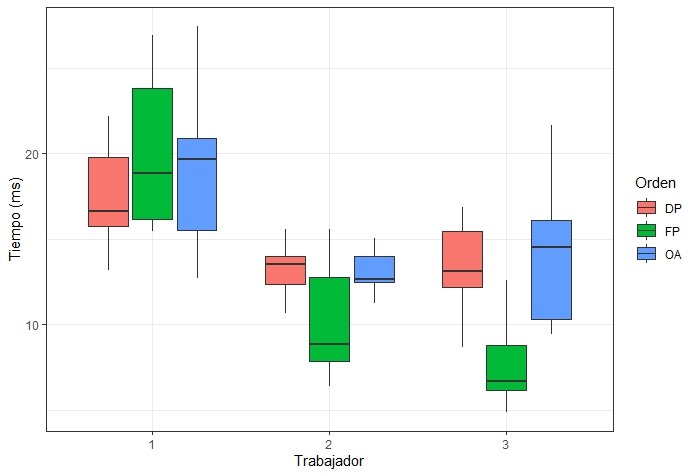
\includegraphics[width=150mm]{Figura1.jpeg} % archivo
    \caption{Tiempo que tarda cada trabajador en realizar las tareas en cada orden: difíciles primero (DP), fáciles primero (FP) y orden aleatorio (OA).}
    \label{Figura 1}
\end{figure} 
    
\smallskip

Se elegió utilizar la prueba estadística ANOVA de una vía, debido a que se quería realizar un análisis paramétrico para comparar más de 2 grupos. Se revisaron diferentes páginas en internet sobre documentación \citep{2}, y video tutoriales \citep{3,4} para aprender a utilizar la prueba estadística elegida \citep{5}.
\bigskip

Se generó el código para aplicar ANOVA de una vía a los datos de cada trabajador y también a los datos de cada tipo de ordenamiento por separado para así analizar sus medias, en la figura \ref{Figura 2} se muestran los diagramas caja-bigote para cada \texttt{trabajador} y \texttt{ordenamiento}. 
\bigskip

Primeramente, se revisaron los supuestos para poder aplicar la prueba estadística ANOVA. En el cuadro \ref{Cuadro 3} se  resumen los resultados. El supuesto outliers se refiere a la cantidad de valores atípicos que existen en los grupos, la normalidad por grupos se obtuvo con la prueba de \texttt{Shapiro Wilk}, y la homogeneidad de varianza se obtuvo con la prueba de \texttt{Levene}.

\begin{table}[ht]
\centering
\caption{Resultados del los supuestos para aplicar la prueba estadística ANOVA.}
\smallskip

\begin{tabular}{ |p{2.1cm}||p{2.1cm}||p{2.1cm}||p{2.1cm}||p{2.1cm}||p{2cm}||p{2cm}|}
 \hline
 & Trabajador 1 & Trabajador 2 & Trabajador 3 & Orden FP & Orden DP & Orden OA\\
 \hline
 Outliers & $0$ & $0$ & $0$ & $0$ & $0$ & $0$ \\
 \hline
 Normalidad por grupo & FP $p$ = $0.190$ DP $p$ = $0.648$ OA $p$ = $0.875$ & FP $p$ = $0.182$ DP $p$ = $0.826$ OA $p$ = $0.610$ & FP $p$ = $0.083$ DP $p$ = $0.807$ OA $p$ = $0.249$ & T1 $p$ = $0.190$ T2 $p$ = $0.182$ T3 $p$ = $0.083$ &  T1 $p$ = $0.648$ T2 $p$ = $0.826$ T3 $p$ = $0.807$ &  T1 $p$ = $0.875$ T2 $p$ = $0.610$ T3 $p$ = $0.249$ \\
 \hline
 Homogeneidad de varianza & $p$ = $0.356$ & $p$ = $0.068$ & $p$ = $0.135$ & $p$ = $0.251$ & $p$ = $0.421$ & $p$ = $0.018$\\
 \hline
\end{tabular}
\label{Cuadro 3}
\end{table}

En el cuadro \ref{Cuadro 3} se puede ver que los valores de $p$ son mayores a $0.05$ por lo cual se cumplen los supuestos, excepto en la homogeneidad de varianza del \texttt{Orden OA}. Para el ordenamiento \texttt{OA} se aplicó la prueba estadística ANOVA de Welch, la cual puede utilizarse cuando no se tiene varianza homogénea.

\newpage
.
\bigskip

\begin{figure} [h!]% figura
    \caption{Tiempos para cada trabajador y cada orden por separado.}
    \smallskip
    \centering
    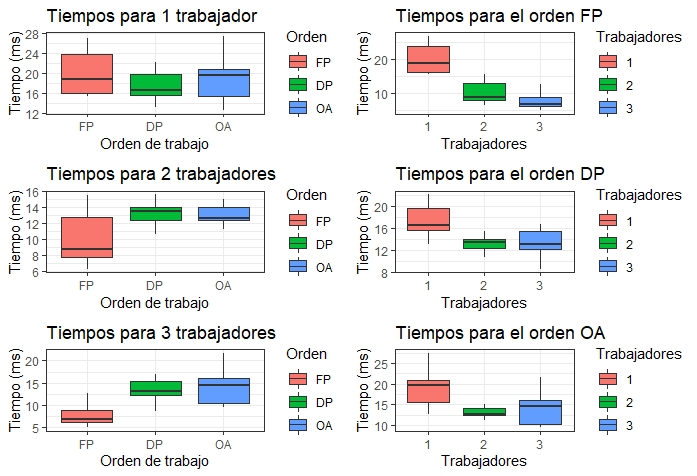
\includegraphics[width=140mm]{Figura2.jpeg} % archivo
    \label{Figura 2}
\end{figure} 

También se calculó la normalidad por residuales y los resultados se muestran en la figura \ref{Figura 3}.

\begin{figure} [h!]% figura
    \caption{Normalidad por residuales.}
    \smallskip
    \centering
    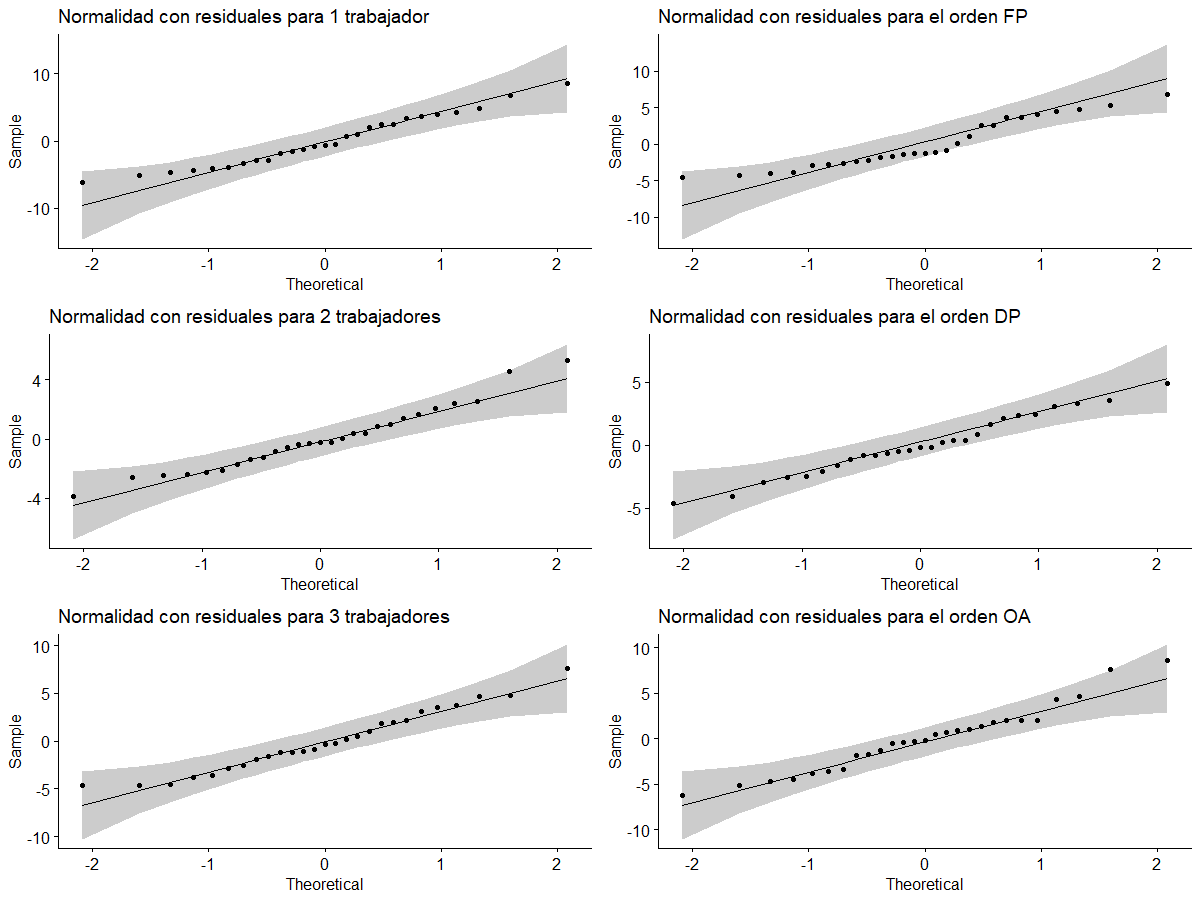
\includegraphics[width=140mm]{Figura3.jpeg} % archivo
    \label{Figura 3}
\end{figure} 

\newpage
.
\bigskip

Los resultados de la normalidad por grupos se muestran en la figura \ref{Figura 4}.

\begin{figure} [h!]% figura
    \caption{Normalidad por grupos separados.}
    \smallskip
    \centering
    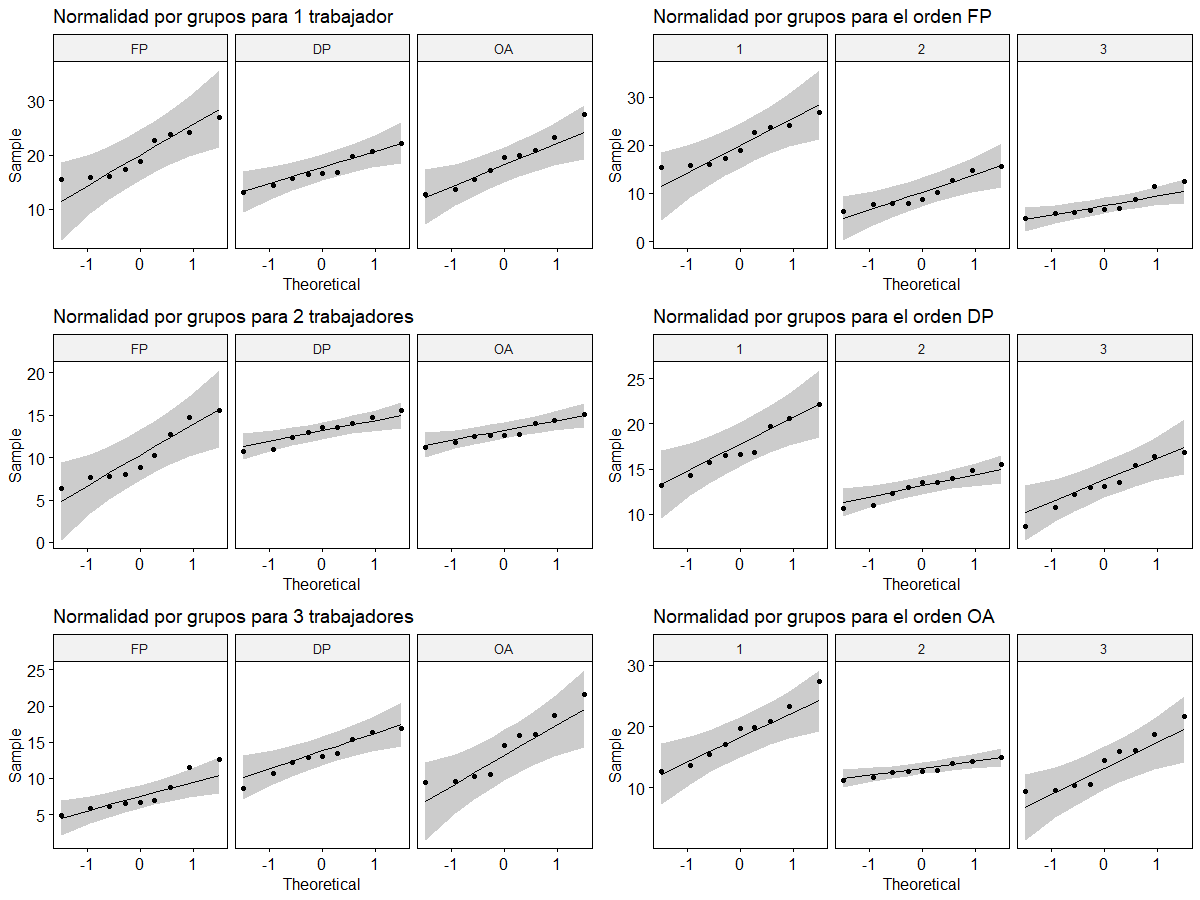
\includegraphics[width=140mm]{Figura4.jpeg} % archivo
    \label{Figura 4}
\end{figure}

A continuación, en el cuadro \ref{Cuadro 4} se muestran los resultados de la prueba estadística ANOVA.

\begin{table}[ht]
\centering
\caption{Resultados de la prueba estadística ANOVA de una vía.}
\smallskip

 \begin{tabular}{ |p{2.2cm}|p{1.8cm}|p{11.5cm}|}
 \hline
 Grupo & Valor de $p$ & Comparaciones múltiples de Tukey de medias (nivel de confianza del 0.95)\\
 \hline
 Trabajador 1  & $0.354$ & DP-FP: $p$ = $0.323$ / OA-FP: $p$ = $0.801$ / OA-DP: $p$ = $0.686$\\
 \hline
 Trabajador 2 & $0.0177$ & DP-FP: $p$ = $0.028$ / OA-FP: $p$ = $0.039$ / OA-DP: $p$ = $0.987$\\
 \hline
 Trabajador 3 & $0.0008$ & DP-FP: $p$ = $0.004$ / OA-FP: $p$ = $0.001$ / OA-DP: $p$ = $0.872$\\
 \hline
 Orden FP & $2.04e-07$  & T2-T1: $p$ = $0.000$ / T3-T1: $p$ = $0.000$ / T3-T2: $p$ = $0.319$ \\
 \hline
 Orden DP & $0.0020$ & T2-T1: $p$ = $0.004$ / T3-T1: $p$ = $0.006$ / T3-T2: $p$ = $0.989$  \\
 \hline
 Orden OA & $0.013$ & T2-T1: $p$ = $0.013$ / T3-T1: $p$ = $0.096$ / T3-T2: $p$ = $0.755$  \\
 \hline
\end{tabular}
\label{Cuadro 4}
\end{table}

Como se mencionó anteriormente para el grupo \texttt{Orden OA} se utilizó la prueba estadística ANOVA de Welch. 
\smallskip

Si tenemos la hípotesis nula siguiente: 
\smallskip

Hípotesis Nula: Las medias de todos los grupos son iguales.
\bigskip

En los resultados mostrados en el cuadro \ref{Cuadro 4} podemos notar que $p < 0.05$ en la mayoría de los grupos, por lo tanto podemos decir que:
\smallskip

Se rechaza la hípostesis nula.

Hípotesis alternativa: Las medias son estadísticamente significativas en los grupos \texttt{Trabajador 2, Trabajador 3, Orden FP, Orden DP y Orden OA },  es decir que en estos grupos las medias sí son diferentes. Solamente en el grupo \texttt{Trabajador 1} se tienen medias no significativas. 
\bigskip

Enseguida se muestra el código generado en \texttt{RStudio} para esta práctica \citep{6}.
\newpage
.
\bigskip

\definecolor{morado}{rgb}{0.34,0.13,0.39}
\definecolor{codegray}{rgb}{0.5,0.5,0.5}
\definecolor{codegreen}{rgb}{0,0.56,0.22}
\definecolor{backcolour}{rgb}{0.95,0.95,0.92}
\definecolor{azul}{rgb}{0,0,1}

\lstdefinestyle{mystyle}{
    backgroundcolor=\color{backcolour},   
    commentstyle=\color{morado},
    keywordstyle=\color{azul},
    numberstyle=\tiny\color{codegray},
    stringstyle=\color{codegreen},
    basicstyle=\ttfamily\footnotesize,
    breakatwhitespace=false,         
    breaklines=true,                 
    captionpos=b,                    
    keepspaces=true,                 
    numbers=left,                    
    numbersep=5pt,                  
    showspaces=false,                
    showstringspaces=false,
    showtabs=false,                  
    tabsize=2
}
\lstset{style=mystyle}
\begin{lstlisting}[language=R, caption= Código para la prueba estadística ANOVA y ANOVA Welch.]
#PRUEBA ESTADISTICA ANOVA
install.packages("tidyverse")
install.packages("ggpubr")
install.packages("rstatix")
install.packages("rapportools")

library(tidyverse)
library(ggpubr)
library(rstatix)
library(rapportools)
library(readr)
library(ggplot2)
library(gridExtra)

ruta_csv = "C:\\Users\\beren\\OneDrive\\Escritorio\\Maestría\\2do semestre\\5. Simulación computacional de nanomateriales\\Tareas\\Tarea_3\\misdatos.csv"

datos = read.csv(ruta_csv)

names(datos) <- c("Replica", "Trabajador", "Orden", "Tiempo")

datos$Trabajador= as.factor(datos$Trabajador) #crear vector a partir del dataframe
datos$Orden = as.factor(datos$Orden) #crear vector a partir del dataframe

ggplot(data = datos, aes(x = Trabajador, y = Tiempo, fill = Orden)) +
  geom_boxplot() + theme_bw() + labs(y = "Tiempo (ms)")


library(readxl)
ruta_excel = "C:/Users/beren/OneDrive/Escritorio/Maestría/2do semestre/5. Simulación computacional de nanomateriales/Tareas/Tarea_3/misdatos.xlsx"
misdatos <- read_excel(ruta_excel)
excel_sheets(ruta_excel)

trabajador1 = read_excel(ruta_excel, sheet = "Trabajador1")
trabajador2 = read_excel(ruta_excel, sheet = "Trabajador2")
trabajador3 = read_excel(ruta_excel, sheet = "Trabajador3")
ordenfp = read_excel(ruta_excel, sheet = "FP")
ordendp = read_excel(ruta_excel, sheet = "DP")
ordenoa = read_excel(ruta_excel, sheet = "OA")


#ANALISIS DESCRIPTIVO
#Un trabajador
trabajador1 = trabajador1 %>%
  rstatix::reorder_levels(Orden, order = c("FP", "DP", "OA"))

trabajador1 %>%
  group_by(Orden) %>%
  get_summary_stats(Tiempo, type = "mean_sd")
#Dos trabajadores
trabajador2 = trabajador2 %>%
  rstatix::reorder_levels(Orden, order = c("FP", "DP", "OA"))

trabajador2 %>%
  group_by(Orden) %>%
  get_summary_stats(Tiempo, type = "mean_sd")
#Tres trabajadores
trabajador3 = trabajador3 %>%
  rstatix::reorder_levels(Orden, order = c("FP", "DP", "OA"))

trabajador3 %>%
  group_by(Orden) %>%
  get_summary_stats(Tiempo, type = "mean_sd")
#Orden FP
ordenfp = ordenfp %>%
  rstatix::reorder_levels(Trabajadores, order = c("1", "2", "3"))

ordenfp %>%
  group_by(Trabajadores) %>%
  get_summary_stats(Tiempo, type = "mean_sd")
#Orden DP
ordendp = ordendp %>%
  rstatix::reorder_levels(Trabajadores, order = c("1", "2", "3"))

ordendp %>%
  group_by(Trabajadores) %>%
  get_summary_stats(Tiempo, type = "mean_sd")
#Orden OA
ordenoa = ordenoa %>%
  rstatix::reorder_levels(Trabajadores, order = c("1", "2", "3"))

ordenoa %>%
  group_by(Trabajadores) %>%
  get_summary_stats(Tiempo, type = "mean_sd")

#VISUALIZAR DATOS
#Un trabajador
g1 = ggplot(data = trabajador1, aes(x = Orden, y = Tiempo, fill = Orden)) + 
  geom_boxplot() + theme_bw() + labs(x = "Orden de trabajo", y = "Tiempo (ms)", title = 'Tiempos para 1 trabajador')

#Dos trabajadores
g2 = ggplot(data = trabajador2, aes(x = Orden, y = Tiempo, fill = Orden)) + 
  geom_boxplot() + theme_bw() + labs(x = "Orden de trabajo", y = "Tiempo (ms)", title = 'Tiempos para 2 trabajadores')

#Tres trabajadores
g3 = ggplot(data = trabajador3, aes(x = Orden, y = Tiempo, fill = Orden)) + 
  geom_boxplot() + theme_bw() + labs(x = "Orden de trabajo", y = "Tiempo (ms)", title = 'Tiempos para 3 trabajadores')

#Orden FP
g4 = ggplot(data = ordenfp, aes(x = Trabajadores, y = Tiempo, fill = Trabajadores)) + 
  geom_boxplot() + theme_bw() + labs(x = "Trabajadores", y = "Tiempo (ms)", title = 'Tiempos para el orden FP')

#Orden DP
g5 = ggplot(data = ordendp, aes(x = Trabajadores, y = Tiempo, fill = Trabajadores)) + 
  geom_boxplot() + theme_bw() + labs(x = "Trabajadores", y = "Tiempo (ms)", title = 'Tiempos para el orden DP')

#Orden OA
g6 = ggplot(data = ordenoa, aes(x = Trabajadores, y = Tiempo, fill = Trabajadores)) + 
  geom_boxplot() + theme_bw() + labs(x = "Trabajadores", y = "Tiempo (ms)", title = 'Tiempos para el orden OA')

grid.arrange(g1, g4, g2, g5, g3, g6, ncol = 2)

#SUPUESTOS PARA ANOVA

#1:OUTLIERS
#Un trabajador
trabajador1 %>%
  group_by(Orden) %>%
  identify_outliers(Tiempo)

#Dos trabajadores
trabajador2 %>%
  group_by(Orden) %>%
  identify_outliers(Tiempo)

#Tres trabajadores
trabajador3 %>%
  group_by(Orden) %>%
  identify_outliers(Tiempo)

#Orden FP
ordenfp %>%
  group_by(Trabajadores) %>%
  identify_outliers(Tiempo)

#Orden DP
ordendp %>%
  group_by(Trabajadores) %>%
  identify_outliers(Tiempo)

#Orden OA
ordenoa %>%
  group_by(Trabajadores) %>%
  identify_outliers(Tiempo)

#2:NORMALIDAD CON RESIDUALES
#Un trabajador
normalidad1 = lm(Tiempo ~ Orden, data = trabajador1)
head(trabajador1)
head(normalidad1$fitted.values)
head(normalidad1$residuals)

n1 = ggqqplot(residuals(normalidad1))+
  labs(title = 'Normalidad con residuales para 1 trabajador')
shapiro_test(residuals(normalidad1))

trabajador1 %>%
  group_by(Orden) %>%
  shapiro_test(Tiempo)

#Dos trabajadores
normalidad2 = lm(Tiempo ~ Orden, data = trabajador2)
head(trabajador2)
head(normalidad2$fitted.values)
head(normalidad2$residuals)

n2 = ggqqplot(residuals(normalidad2))+
  labs(title = 'Normalidad con residuales para 2 trabajadores')
shapiro_test(residuals(normalidad2))

trabajador2 %>%
  group_by(Orden) %>%
  shapiro_test(Tiempo)

#Tres trabajadores
normalidad3 = lm(Tiempo ~ Orden, data = trabajador3)
head(trabajador3)
head(normalidad3$fitted.values)
head(normalidad3$residuals)

n3 = ggqqplot(residuals(normalidad3))+
  labs(title = 'Normalidad con residuales para 3 trabajadores')
shapiro_test(residuals(normalidad3))

trabajador3 %>%
  group_by(Orden) %>%
  shapiro_test(Tiempo)

#Orden FP
normalidad4 = lm(Tiempo ~ Trabajadores, data = ordenfp)
head(ordenfp)
head(normalidad4$fitted.values)
head(normalidad4$residuals)

n4 = ggqqplot(residuals(normalidad4))+
  labs(title = 'Normalidad con residuales para el orden FP')
shapiro_test(residuals(normalidad4))

ordenfp %>%
  group_by(Trabajadores) %>%
  shapiro_test(Tiempo)

#Orden DP
normalidad5 = lm(Tiempo ~ Trabajadores, data = ordendp)
head(ordendp)
head(normalidad5$fitted.values)
head(normalidad5$residuals)

n5 = ggqqplot(residuals(normalidad5))+
  labs(title = 'Normalidad con residuales para el orden DP')
shapiro_test(residuals(normalidad5))

ordendp %>%
  group_by(Trabajadores) %>%
  shapiro_test(Tiempo)

#Orden OA
normalidad6 = lm(Tiempo ~ Trabajadores, data = ordenoa)
head(ordenoa)
head(normalidad6$fitted.values)
head(normalidad6$residuals)

n6 = ggqqplot(residuals(normalidad6))+
  labs(title = 'Normalidad con residuales para el orden OA')
shapiro_test(residuals(normalidad6))

ordenoa %>%
  group_by(Trabajadores) %>%
  shapiro_test(Tiempo)

grid.arrange(n1, n4, n2, n5, n3, n6, ncol = 2)

#NORMALIDAD PARA CADA GRUPO POR SEPARADO
#Un trabajador
m1 = ggqqplot(data = trabajador1, x = "Tiempo", facet.by = "Orden")+
  labs(title = 'Normalidad por grupos para 1 trabajador')
trabajador1 %>%
  group_by(Orden) %>%
  shapiro_test(Tiempo)

#Dos trabajadores
m2 = ggqqplot(data = trabajador2, x = "Tiempo", facet.by = "Orden")+
  labs(title = 'Normalidad por grupos para 2 trabajadores')
trabajador2 %>%
  group_by(Orden) %>%
  shapiro_test(Tiempo)

#Tres trabajadores
m3 = ggqqplot(data = trabajador3, x = "Tiempo", facet.by = "Orden")+
  labs(title = 'Normalidad por grupos para 3 trabajadores')
trabajador3 %>%
  group_by(Orden) %>%
  shapiro_test(Tiempo)

#Orden FP
m4 = ggqqplot(data = ordenfp, x = "Tiempo", facet.by = "Trabajadores")+
  labs(title = 'Normalidad por grupos para el orden FP')
ordenfp %>%
  group_by(Trabajadores) %>%
  shapiro_test(Tiempo)

#Orden DP
m5 = ggqqplot(data = ordendp, x = "Tiempo", facet.by = "Trabajadores")+
  labs(title = 'Normalidad por grupos para el orden DP')
ordendp %>%
  group_by(Trabajadores) %>%
  shapiro_test(Tiempo)

#Orden OA
m6 = ggqqplot(data = ordenoa, x = "Tiempo", facet.by = "Trabajadores")+
  labs(title = 'Normalidad por grupos para el orden OA')
ordenoa %>%
  group_by(Trabajadores) %>%
  shapiro_test(Tiempo)

grid.arrange(m1, m4, m2, m5, m3, m6, ncol = 2)

#HOMOGENEIDAD DE VARIANZAS CON PRUEBA DE LEVENE
#Un trabajador
trabajador1 %>%
  levene_test(Tiempo~Orden)

#Dos trabajadores
trabajador2 %>%
  levene_test(Tiempo~Orden)

#Tres trabajadores
trabajador3 %>%
  levene_test(Tiempo~Orden)

#Orden FP
ordenfp %>%
  levene_test(Tiempo~Trabajadores)

#Orden DP
ordendp %>%
  levene_test(Tiempo~Trabajadores)

#Orden OA
ordenoa %>%
  levene_test(Tiempo~Trabajadores)

#ANOVA
#Un trabajador
view(trabajador1)
trabajador1
attach(trabajador1)
names(trabajador1)
class(Orden)
class(Tiempo)
summary(trabajador1)
boxplot(Tiempo~Orden)
aov(Tiempo~Orden)
anova1 = aov(Tiempo~Orden)
summary(anova1)
TukeyHSD(anova1)

#Dos trabajadores
view(trabajador2)
trabajador2
attach(trabajador2)
names(trabajador2)
class(Orden)
class(Tiempo)
summary(trabajador2)
boxplot(Tiempo~Orden)
aov(Tiempo~Orden)
anova2 = aov(Tiempo~Orden)
summary(anova2)
TukeyHSD(anova2)

#Tres trabajadores
view(trabajador3)
trabajador3
attach(trabajador3)
names(trabajador3)
class(Orden)
class(Tiempo)
summary(trabajador3)
boxplot(Tiempo~Orden)
aov(Tiempo~Orden)
anova3 = aov(Tiempo~Orden)
summary(anova3)
TukeyHSD(anova3)

#Orden FP
view(ordenfp)
ordenfp
attach(ordenfp)
names(ordenfp)
class(Trabajadores)
class(Tiempo)
summary(ordenfp)
boxplot(Tiempo~Trabajadores)
aov(Tiempo~Trabajadores)
anova4 = aov(Tiempo~Trabajadores)
summary(anova4)
TukeyHSD(anova4)

#Orden DP
view(ordendp)
ordendp
attach(ordendp)
names(ordendp)
class(Trabajadores)
class(Tiempo)
summary(ordendp)
boxplot(Tiempo~Trabajadores)
aov(Tiempo~Trabajadores)
anova5 = aov(Tiempo~Trabajadores)
summary(anova5)
TukeyHSD(anova5)

#ANOVA DE WELCH
#Orden OA
anova6 = ordenoa %>% welch_anova_test(Tiempo~Trabajadores)
anova6
comp_mult = ordenoa %>% games_howell_test(Tiempo~Trabajadores)
comp_mult

\end{lstlisting}

Después de revisar otras páginas de internet y video tutoriales \citep{7}, encontré que para analizar el efecto de los trabajadores y el orden de los trabajos en una sola prueba estadística se puede utilizar ANOVA para dos vías o factores. Para esta prueba también se revisó la homogeneidad de varianza con una prueba de \texttt{Levene} y la normalidad con una prueba de \texttt{Shapiro Wilk}. Los resultados se muestran en el cuadro \ref{Cuadro 5}, e indican que ambos resultados no son significativos, es decir que si hay normalidad y varianza homogénea.

\begin{table}[ht]
\centering
\caption{Resultados de pruebas de varianza y normalidad.}
\smallskip

 \begin{tabular}{ |p{2.5cm}|p{1.5cm}|}
 \hline
 Prueba & $p$ \\
 \hline
 \texttt{Levene} & $0.1648$ \\
 \hline
 \texttt{Shapiro Wilk}  & $0.1069$ \\
 \hline
\end{tabular}
\label{Cuadro 5}
\end{table}

En el código se realizaron dos modelos para la prueba estadística, el \texttt{Modelo 1} de ANOVA que es para solo considerar efectos principales de las variables independientes \texttt{Trabajador} y \texttt{Orden}, y el \texttt{Modelo 2} toma en cuenta las interacciones que existen entre dichas variables. Si el resultado del \texttt{Modelo 2} es significativo se debe realizar un análisis de ANOVA \texttt{Tipo III} , y de lo contrario se utiliza un \texttt{Tipo II}. En los cuadros \ref{Cuadro 6} y \ref{Cuadro 7} se presentan los resultados de los modelos, los cuales indican que la interacción entre las dos variables si es significativa.

\begin{table}[ht]
\centering
\caption{Resultados del Modelo 1.}
\smallskip

 \begin{tabular}{ |p{2.5cm}|p{1.7cm}|}
 \hline
 Variables & $p$ \\
 \hline
 \texttt{Trabajador} & $1.758e-09$ \\
 \hline
 \texttt{Orden}  & $0.118$ \\
 \hline
\end{tabular}
\label{Cuadro 6}
\end{table}

\begin{table}[ht]
\centering
\caption{Resultados del Modelo 2.}
\smallskip

 \begin{tabular}{ |p{3cm}|p{2cm}|}
 \hline
 Variables & $p$ \\
 \hline
 \texttt{Trabajador} & $5.845e-10$ \\
 \hline
 \texttt{Orden}  & $0.09832$ \\
 \hline
  \texttt{Orden:Trabajador}  & $0.03684$ \\
 \hline
\end{tabular}
\label{Cuadro 7}
\end{table}


\newpage

Realizando la prueba estadística de ANOVA de dos factores \texttt{Tipo III} se obtienen los resultados mostrados en el cuadro \ref{Cuadro 8}.

\begin{table}[ht]
\centering
\caption{Resultados de pruebas estadística ANOVA de dos factores}
\smallskip

 \begin{tabular}{ |p{3cm}|p{1.7cm}|p{6cm}|}
 \hline
 Variables & $p$ & Interpretación \\
 \hline
 \texttt{Trabajador} & $5.845e-10$ & $p < 0.05$ entonces es significativa\\
 \hline
 \texttt{Orden}  & $0.09832$ & $p > 0.05$ entonces no es significativa \\
 \hline
  \texttt{Orden:Trabajador}  & $0.036842$ & $p < 0.05$ entonces es significativa \\
 \hline
\end{tabular}
\label{Cuadro 8}
\end{table}

Hipótesis nula: Las medias son iguales en todos los grupos.
\smallskip

Hipótesis alternativa: Se rechaza la hipótesis nula. Si existen diferencias en los tiempos de los trabajadores, es decir que el tiempo se ve afectado por el hecho de asignar más núcleos en el cluster. Y en cuanto al orden en que se realizan los trabajos si afecta de manera significativa en los tiempos cuando se tiene la interacción con los diferentes trabajadores.

El código generado para la prueba estadística ANOVA con dos factores se muestra a continuación: 

\definecolor{codered}{rgb}{1,0,0}
\definecolor{codegray}{rgb}{0.5,0.5,0.5}
\definecolor{codegreen}{rgb}{0,0.56,0.22}
\definecolor{backcolour}{rgb}{0.95,0.95,0.92}
\definecolor{naranja}{rgb}{0.92,0.48,0.15}

\lstdefinestyle{mystyle}{
    backgroundcolor=\color{backcolour},   
    commentstyle=\color{codered},
    keywordstyle=\color{naranja},
    numberstyle=\tiny\color{codegray},
    stringstyle=\color{codegreen},
    basicstyle=\ttfamily\footnotesize,
    breakatwhitespace=false,         
    breaklines=true,                 
    captionpos=b,                    
    keepspaces=true,                 
    numbers=left,                    
    numbersep=5pt,                  
    showspaces=false,                
    showstringspaces=false,
    showtabs=false,                  
    tabsize=2
}
\lstset{style=mystyle}
\begin{lstlisting}[language=R, caption= Código para prueba estadística ANOVA de dos vías.]
install.packages("car")
install.packages("reshape")
install.packages("multcomp")
install.packages("pastecs")
install.packages("WRS")

library(ggplot2)
library(car)
library(reshape)
library(multcomp)
library(pastecs)
library(WRS)
library(tidyverse)
library(ggpubr)
library(rstatix)
library(rapportools)
library(readr)
library(ggplot2)
library(gridExtra)

names(misdatos2)

misdatos2$Trabajador= as.character(misdatos2$Trabajador) #crear vector a partir del dataframe
misdatos2$Orden = as.character(misdatos2$Orden) #crear vector a partir del dataframe
misdatos2$Tiempo = as.numeric(misdatos2$Tiempo) #crear vector a partir del dataframe

attach(misdatos2)
names(misdatos2)

class(Trabajador)
class(Orden)
class(Tiempo)
factor(Trabajador)
factor(Orden)

leveneTest(misdatos2$Tiempo, interaction(misdatos2$Orden, misdatos2$Trabajador), center = median)

Model1 = aov(Tiempo~Trabajador+Orden, data = misdatos2) #Modelo con efectos principales
anova(Model1)

Model2 = aov(Tiempo~Orden*Trabajador, data = misdatos2) #Modelo con efectos principales con interacción
anova(Model2)

plot(Model1)

aov_residuals = residuals(object = Model1)
shapiro.test(x=aov_residuals)

Anova(Model2, Type = "III")


\end{lstlisting}

\newpage
.
\bigskip

\section{Conclusi\'{o}n}
Con base en los resultados obtenidos de las diferentes pruebas estadísticas ANOVA que realicé puedo concluír que cuando se asigan más núcleos en el cluster el trabajo o la tarea se puede realizar más rápidamente. En general el desarrollo de la práctica me aportó conocimiento sobe las diferentes pruebas estadísticas, los requerimientos que tiene cada una de ellas y sus aplicaciones. 

\newpage
.
\bigskip
\bigskip


\bibliography{referencias}
\bibliographystyle{plainnat}

\end{document}